\chapter{Clustering}
\emph{Clustering} analysis relate to finding groups of objects such that the objects in a group will be similar (or related) to one another 
and different from (or unrelated to) the objects in other groups, as it is possible to note in figure \ref{img:cluster}

\begin{figure}
    \caption{Cluster Example}
    \label{img:cluster}
    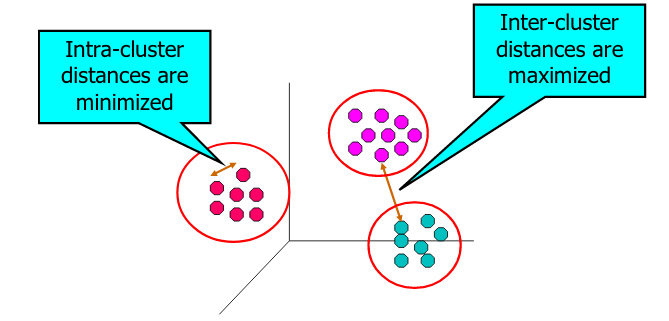
\includegraphics[width=\textwidth]{Images/cluster}
\end{figure}

\begin{figure}
    \caption{Ambiguity about number of Cluster}
    \label{img:ambiguousCluster}
    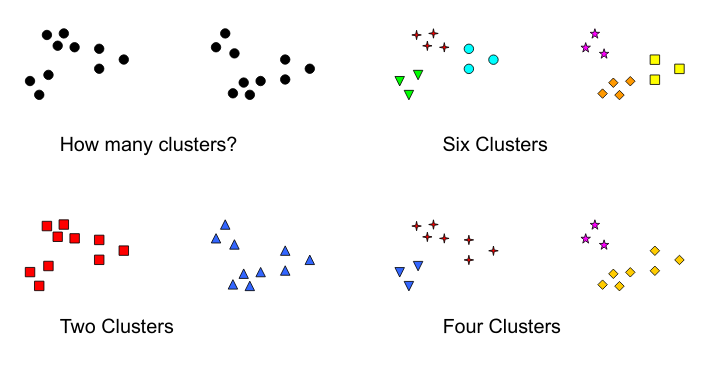
\includegraphics[width=\textwidth]{Images/anomoulous}
\end{figure}

The notion of cluster can be ambiguous as can be note in figure \ref{img:ambiguousCluster} and a clustering is a set of clusters, where exist
an important distinction between:
\begin{description}
    \item [Partitional Clustering: ] a division of data objects into non-overlapping subsets (clusters) such that each data object is in exactly one subset
    				     as can be viewed in figure \ref{img:partitionalCluster}.

				     \begin{figure}
				         \caption{Example of Partitional Clustering}
					 \label{img:partitionalCluster}
					 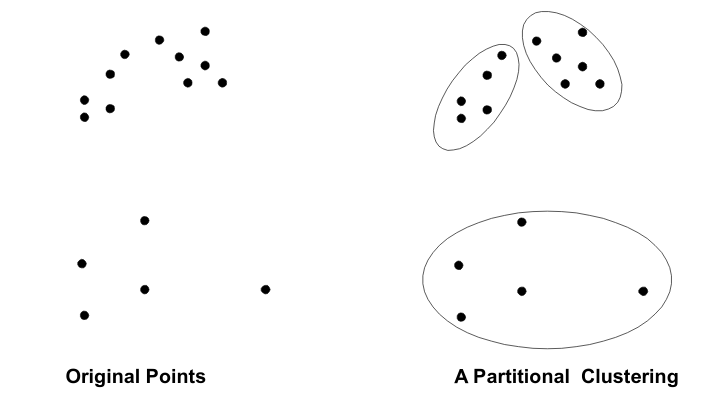
\includegraphics[width=\textwidth]{Images/partitional}
				     \end{figure}

    \item [Hierarchical Clustering: ] a set of nested clusters organized as a hierarchical tree, as can be note in figure \ref{img:hierarchicalCluster}.

    				      \begin{figure}
				          \caption{Example of Hierarchical Clustering}
					  \label{img:hierarchicalCluster}
					  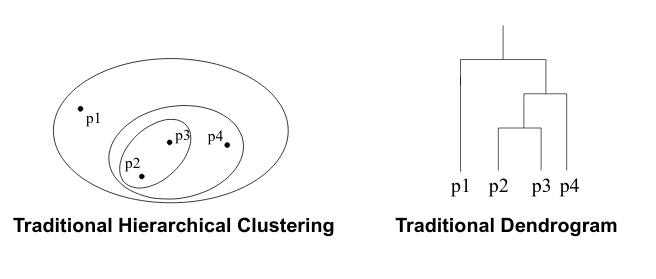
\includegraphics[width=\textwidth]{Images/hierarchical}
				      \end{figure}
\end{description}
We have the following type of Clusters:
\begin{description}
    \item [Well-Separated Clusters: ] is a set of points such that any point in a cluster is closer (or more similar) to every other point in the cluster than to any point not in the cluster

    \item [Center-based Clusters: ] is a set of objects such that an object in a cluster is closer (more similar) to the “center” of a cluster, than to the center of any other cluster; 
	                            the center of a cluster is often a \emph{centroid}, the average of all the points in the cluster, or a \emph{medoid}, the most “representative” point of a cluster.

    \item [Contiguous Cluster (Nearest neighbor or Transitive): ] each point is closer to at least one point in its cluster than to any point in another cluster and 
	                                                          this approach can have trouble when noise is present since a small bridge of points can merge two distinct clusters.

    \item [Density-based: ] is a dense region of points, which is separated by low-density regions, from other regions of high density and used when the clusters are irregular or intertwined, and when noise and outliers are present.
\end{description}
Clusters are defined by an Objective Function, so we Finds clusters that minimize/maximize an objective function and enumerate all possible ways of dividing the points into clusters and evaluate the `goodness' of each potential
set of clusters by using the given objective function is an NP Hard problem.\newline
There can be global or local objectives: Hierarchical clustering algorithms typically have local objectives, instead Partitional algorithms typically have global objectives.


